\chapter{Theory}

\cite{goodman2000,goodman2007,agarwal2013,classen2017,goodman2000,cowley1995,born1980,trigg2005,attwood1999,griffiths2005,goodman2007,agarwal2013,classen2017,loudon2000,mandel1995,hanburry1956,galuber2006,baym1997,zernike1938,rosen96,yabashi2002,singer2013,santra2009,krause1979,trost2020,inoue2019,sorum1987,lajunen04,mpccd,tono2013}

random process
ergodic: time average equals expectation value
stationary: shifting all time instants by $\tau$ does not change the statistical description of the random process 

\section{Coherence}
Spherical waves as  solutions to wave equation
\begin{equation}
	E(\vec{r},t)=E_0(k,t) \frac{e^{i\vec{r}\vec{k}-iwt}}{R}
	\end{equation}

Superposition principle of the waves with the real amplitudes $A_{1,2}$ and phases $\phi{1,2}$
\begin{equation}
E(\vec{r},t)=E_1(\vec{r},t)+E_2\vec{r},t)=A_1*e^{i\phi_1} * e^{i\vec{r}\vec{k_1}-iw_1t} + A_1*e^{i\phi_1} * e^{i\vec{r}\vec{k_2}-iw_2t} 
\end{equation} 

measured Intensity with measurement time $T\gg1/w$
\begin{equation}
	I(\vec{r},t)\propto \int_0^T \left|E(\vec{r},t)\right|^2 \diff t
\end{equation}
Consider monochromatic light

Superposition of two monochromatic, stationary waves with a fixed phase difference $\Delta \phi$ gives rise to interference fringes
\begin{equation}
	\left<I(\vec{r},t)\right>=I_1+I_2+2\sqrt{I_1I_2}\cos\left((\vec{k_1}-\vec{k_2})\vec{r}+\Delta \phi\right)
\end{equation}

Defining the contrast of the fringes as the visibility $V$,
\begin{equation}
	V=\frac{I_{max}-I_{min}}{I_{max}+I_{min}}
\end{equation} 

Gives $V=\frac{2\sqrt{I*I}}{I+I}I=1$.

To consider non monochromatic waves we define self coherence function $\Gamma$ as 
\begin{equation}
\Gamma(\tau)=\left< E(t)E(t+\tau)\right>
\end{equation}
and its normalized version, the complex degree of coherence $\gamma$ as
\begin{equation}
\gamma(\tau)=\frac{\Gamma(\tau)}{\Gamma(0)} =  \frac{\Gamma(\tau)}{<I>}
\end{equation}



The coherence time is defined as 
\begin{equation}
\tau_c = \int_{-\infty}^{\infty} \left| g^1(\tau)\right|^2 \diff \tau 
\end{equation}





\paragraph{First order coherence $g_1$}
Generalization of$\gamma$  for to different fields  $E_1^*(\vec{r}_1,t_1)$ and $E_2(\vec{r}_2,t_2)$ is $g_1$
\begin{equation}
	g^{(1)}(\vec{r}_1,t_1;\vec{r}_2,t_2= \frac
	{\left< E_1^*(\vec{r}_1,t_1)E_2(\vec{r}_2,t_2) \right>}
	{\left[ \left<\left | E(\vec{r}_1,t_1)\right |^2 \right> \left< \left |E(\vec{r}_2,t_2)\right |^2 \right>\right]^{1/2}}	
\end{equation}






In an interferometer, light coming from a source and a time delayed copy are superposed.



For an exponentially decaying electric field $E(t)=\Theta(t)e^{-t/\tau}$, the spectrum is Lorentian with an angular frequency FWHM of $\frac{2}{\tau}$ as 
\begin{equation*}
\left|\int_{0}^{\infty}  e^{-t/\tau} e^{-iwt} \dif t \right|^2 \propto  \frac{1}{1/\tau^2+w^2} .
\end{equation*}
Therefore, an Lorentian spectrum with a FWHM of $\Delta E$ corresponds to an lifetime of $\frac{2\hbar}{\Delta E}$.

Wiener Khinchin to get g1

On the other hand, for a Lorentzian light source, $<g_1(\tau)>=e^{-|\tau/| \tau_c}$, defining the coherence time $\tau_c$ as the time, after which $g^1$ has decreased to $e^{-1} g^1(0)$.

 \begin{figure}
	\centering
	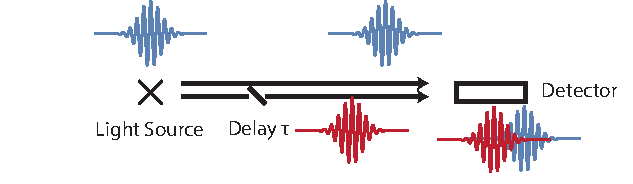
\includegraphics[width=0.8\linewidth]{images/michelson.pdf}
	\caption{Schematic of interferometer: Light of (gaussian) a gaussian light source with finite coherence time is split and interference with a delayed copy is observed. The time averaged intensity meassured by an detector changes with the delay time. }
	\label{fig:michelson}
\end{figure}

\begin{equation}
V=\left|g_1\right|
\end{equation}

Int
-along Glauber/Statistical Optics Goodman



Intensity in double slit leads to normalized degree of coherence $g_1$
Visiblity is modulus of $g_1$.

In a double slit setup (\fref{fig:doubleslit}), $E(r,t)=c_1 E_1(t)+c_2E2(t)$ with complex $c_2$ and $c_2$, $\left|c_1\right|\approx\left|c_2\right|$ describing the propagation to the screen. 

\begin{figure}
	\centering
	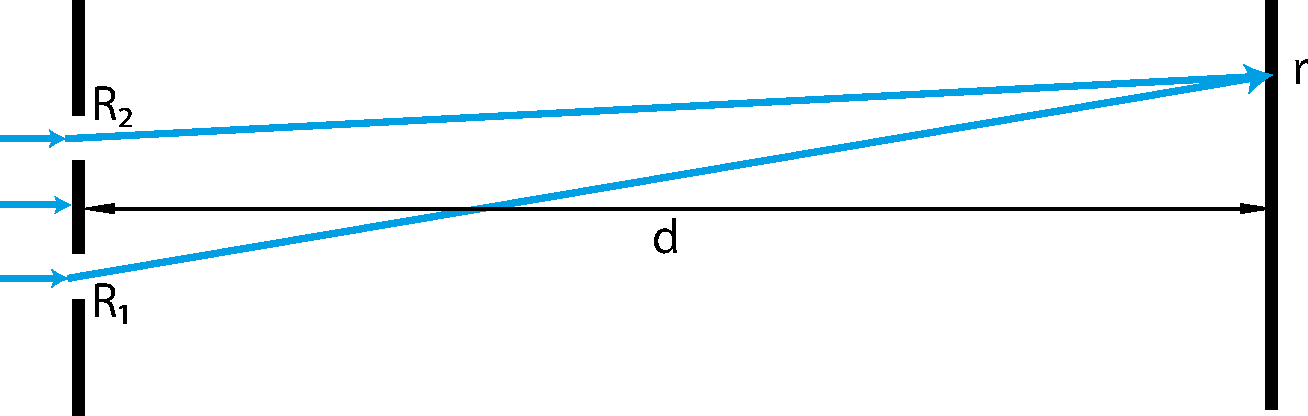
\includegraphics[width=0.8\linewidth]{images/doubleslit.pdf}
	\caption{Schematic of double slit: Monochromatic light goes through slits located at $R_1$ and $R_2$. The intensity at a position $r$ on the scree (in distance $d$) is the superposition of both paths.  If the slits are within the lateral coherence area of the source, the visibility of the interference pattern depends on the path length difference in comparison to the coherence time $\tau$.}
	\label{fig:doubleslit}
\end{figure}


\paragraph{Second order coherence $g_2(t_1,t_2)$}
The definition of $g_1$ can be extended to the second order by
\begin{equation*}
	g^{(2)}(\vec{r}_1,t_1;\vec{r}_2,t_2= 
	\frac{\left< E^*(\vec{r}_1,t_1)E^*(\vec{r}_2,t_2)E(\vec{r}_1,t_1)E(\vec{r}_2,t_2) \right>}{\left<\left | E(\vec{r}_1,t_1)\right |^2 \right> \left< \left |E(\vec{r}_2,t_2)\right |^2 \right>}	
\end{equation*}
For classical fields normalized correlations of intensities:
\begin{equation}
	g^{(2)}(\vec{r}_1,t_1;\vec{r}_2,t_2)= 
		\frac{\left< I(\vec{r}_1,t_1)I(\vec{r}_2,t_2 \right>}{\left<I(\vec{r}_1,t_1)\right>\left<I(\vec{r}_1,t_1)\right>}	
\end{equation}

\paragraph{Van Cittert Zernicke}

%-Hanbury Brown and Twist
\section{Hanburry Brown Twiss}
Hanburry Brown and Twiss 


\paragraph{Siegert Relation for Pseudo-Thermal Light}

%-Single Photon Emitters/2nd Quant description
%(siehe Referenzen in Schaller/resonance fluorescence)
%-Fluorescence g2
%$2 Level with finite Lifetime -> Spectrum of fluorescence
\section{X-Ray Fluorescence}

\section{Intensity Correlations using X-Ray Fluorescence}
\section{Signal to Noise Considerations}
The speckle contrast is governt by the number of independent modes overlaid in the measurement.

Number of temporal degrees of freedom
\begin{equation}
M_t=\frac{\left(\int_{-\infty}^{\infty} P(t)\diff t\right)^2}{\int_{-\infty}^{\infty} K(t) \left|\mu(t)\right|^2\diff t}
\end{equation}
with $P(t)$ the integration window weighting function and $K(t)$ its autocorrelation. If the integration windows is set by the integration time $T$ of the detector, $P(t)$ is a rectangular function with the width $T$ and
\begin{equation}
M_t,rect = \frac{T}{2} \left[\int_{0}^{T} \left( 1-\frac{t}{T}\right) \left|\mu(t)\right|^2 \diff t \right]^{-1} .
\end{equation}
If $P(t)$ is the Gaussian excitation pulse with FWHM of $\tau$ and unit area,
\begin{align}
P(t)&=\frac{2\sqrt{\ln 2}}{\sqrt{\pi} \tau} e^{-\left(2\sqrt{\ln 2}\frac{t}{\tau}\right)^2}\\
K(t)&= \sqrt{\frac{2{\ln 2}}{\pi}}\frac{1}{ \tau} e^{-\left(\sqrt{2\ln 2}\frac{t}{\tau}\right)^2}
\end{align}
and the spectrum is Lorentzian fluorescence, the number of degrees of freedom is
\begin{align}
M_t,gauss&=\left[\int_{-\infty}^{\infty} K(t) \left|\mu(t)\right|^2\diff t\right]^{-1}\\
=42
\end{align}

The experimentally indistinguishable fluorescence energies $K_alpha,1$ and $K_alpha,2$ (as well as  $K_beta$ if no filter is used for suppression) give additional independent modes $M_E$

As the used X-ray detectors are polarization insensitive and X-ray fluorescence is unpolarized, there are 2 independent polarization modes giving $M_P = 2$  


As good approximation, the total number of modes can be considered the product of those modes numbers (in reality, the mode numbers are not completely independent as)
%- SNR
%will use Peak/stdev bg definition
Which factors influence SNR
-lifetime/pulsewidth
-polarisation
-sampling conditions / undersampling
-sample thickness / coherence length
-N images
-N photons
\label{chap:theory}

\section{Kossel Lines}

